\documentclass[12pt, a4]{report}
\usepackage[utf8]{inputenc}
\usepackage[margin=0.8in]{geometry}
\def\thesection{\arabic{section}}
\setcounter{tocdepth}{4}

%
% ─── IMPORTS ────────────────────────────────────────────────────────────────────
%
\usepackage{graphicx}
\graphicspath{ {images/} }
\usepackage{listings}
\usepackage{verbatim}
\usepackage{color}
\usepackage{csquotes}
\usepackage{opensans}

%
% ─── TABLE CONFIGURATIONS ───────────────────────────────────────────────────────
%
\setlength{\arrayrulewidth}{0.5mm}
\setlength{\tabcolsep}{10pt}
\renewcommand{\arraystretch}{1.5}

%
% ─── STYLING AND CONFIGURATION FOR CODE LISTING ─────────────────────────────────
%
\definecolor{codegreen}{rgb}{0,0.6,0}
\definecolor{codegray}{rgb}{0.5,0.5,0.5}
\definecolor{codepurple}{rgb}{0.58,0,0.82}
\definecolor{backcolour}{rgb}{0.95,0.5,0.92}
\definecolor{bittersweet}{rgb}{1.0, 0.44, 0.37}
\definecolor{cosmiclatte}{rgb}{0.93, 0.93, 0.93}
\definecolor{eggshell}{rgb}{0.94, 0.94, 0.9}
\definecolor{fandango}{rgb}{0.71, 0.2, 0.54}
% \definecolor{fawn}{rgb}{0.9, 0.67, 0.44}
\definecolor{fawn}{rgb}{0.89, 0.45, 0.36}
\lstdefinestyle{mystyle}{
	backgroundcolor=\color{cosmiclatte},   
	commentstyle=\color{codegreen},
	keywordstyle=\color{fandango}\small,
	numberstyle=\tiny\color{codegray},
	stringstyle=\color{codepurple},
	basicstyle=\ttfamily\footnotesize,
	breakatwhitespace=false,        
	breaklines=true,               
	captionpos=b,                    
	keepspaces=true,  
	numbers=left,                    
	numbersep=5pt,                  
	showspaces=false,                
	showstringspaces=false,
	showtabs=false,                  
	tabsize=2
}
\lstset{style=mystyle}

%
% ─── COVERPAGE ──────────────────────────────────────────────────────────────────
%
\title{2805, Principles of Software Engineering Milestone 02}
\author{Zaymon Foulds-Cook, s5017391}%\thanks{}}
\date{\today}
\begin{document}
\begin{titlepage}
	\maketitle
\end{titlepage}

\tableofcontents
\pagebreak

%
% ─── START OF REPORT ────────────────────────────────────────────────────────────
%
\section{Principles of Software Engineering Milestone 02}
\subsection{Requirements}
\par Throughout this software project various software requirements have been identified. The following list itemizes each requirement and discusses the current completion status of each item.
\begin{itemize}
	% \par \textcolor{codegreen}{Implemented - ongoing \textbar{} } 
	\item Create system models for structure and behaviour of software products.
	\par \textcolor{codegreen}{Implemented - ongoing \textbar{} } Various models have been created of the software system which allow team members to make architectural decisions as well as gain high level overviews of the software system.
	
	\item Select appropriate software architecture
	\par \textcolor{codegreen}{Implemented - ongoing \textbar{} } The model view controller architecture was chosen for this project and has been fully implemented. The software systems adheres strictly to MVC for interactions, data flow and structure. 

	\item Make use of appropriate design patterns
	\par \textcolor{codegreen}{Implemented - ongoing \textbar{} } Various software design patterns have been used throughout the project such as the `façade software pattern' and the `model view controller pattern'. More patterns such as singleton will be implemented in the final software system.

	\item Create user interface software using event driven or call-back based designs
	\par \textcolor{codegreen}{Implemented - ongoing \textbar{} } The software system has a user interface which is driven by call-back based interactions with the game board.

	\item Create a model `state' representation of the minesweeper game which is generalizable to many different configurations of the minesweeper such as `hex-mines' and `colour-mode'
	\par \textcolor{fawn}{Implemented - to be extended \textbar{} } The board model in the program is generalizable to many different configurations but the hex and colour mode specific implementation is not completed. However, the board state is very versatile and extensible and further implementations should be easily introduced.

	\item Create a controller object which mutates the game state
	\par \textcolor{codegreen}{Implemented - Complete \textbar{} } The game controller is full completed.

	\item Create a main menu which allows the user to select the game mode and difficulty
	\par \textcolor{fawn}{Implemented - to be extended \textbar{} } The main menu currently starts a game correctly and passes parameters back to the parent object on destruction. The main menus functionality will be completed soon when the final game modes are implemented.

	\item Create reusable GUI components
	\par \textcolor{codegreen}{Implemented - ongoing \textbar{} } The main menu, view, and menu bar objects all extend Frame and can be reused.

	\item Create an extensible view object which can adapt to multiple different implementations of the minesweeper game
	\par \textcolor{fawn}{Implemented - to be extended \textbar{} } The current view object uses the model and controller to draw images to the canvas. The view is easily extended and implementing the remaining game modes is straightforward. The current view works for the square implementation of the minesweeper game.
\end{itemize}

\subsection{Product Use Cases}
\par Various use cases were identified in the first milestone. Including:
\begin{itemize}
	\item Select Game Mode
	\item Uncover a tile
	\item Cover a tile
	\item Win the game
	\item Lose the game
\end{itemize}
Most of these use cases have been fully implemented apart from the ability to choose game modes. This use case will be completed with the final project submission as it requires the view and model classes to be extended in order to support the additional game modes. The extension of these classes is covered in section 1.5 `Summary of Design'

\subsection{Summary of Software Architecture}
\par Software architecture is a set of guidelines principles models and processes. The software architecture being used in the minesweeper software system is based around the model view controller software pattern. The Minesweeper software system has been written and implemented purely in python and uses the tkinter user interface library which comes bundled with a typical install of python. No integrated development environments have been used throughout the development process as the developer has opted to simply use the Visual Studio code text editor. 
\newline
\par The modules and components of the Minesweeper software system have been structured in a manner to: reduce coupling, increase cohesion, increase modularity and to enforce a clear separation of concerns between logically related collections of code. The main class of the game MineSweeper is the overarching class and contains objects of the model view and controller classes. The model class represents the internal game-state and does not have a reference to any other class. The controller class is responsible for mutating data in the model by calling the models mutator functions. The controller class does not have a reference to the view. Review class has a reference to both of the controller and the model. The view gets the current state of the model and displays it to the user via a graphical representation. When handling and call back event the view interacts with the model through the controller and the controller acts like a thin proxy or API for the model. This separation between view model and controller allows the internal representation to be changed without impacting interactions between the view and the model. 
\newline
\par The software architecture used in this project enforces modularity by design and allows for a clear separation of concerns. It is highly feasible that the software architecture will remain the same until the project completion as the software architecture allows for highly extendable code and changes can be easily made without cascading changes being needed throughout the project source.

\subsection{Summary of Design}
\par Since milestone 1 it has become apparent that some design goals needed to be created in order to improve the overall effectiveness of the software system in terms of code quality, maintainability and structure. The design goals chosen for the project are: minimising coupling, maximising cohesion, optimising response time, facilitating maintenance and increasing modularity.
\subsubsection{Minimising Coupling}
The original software system for the Milestone 1 submission demonstrated had high levels of coupling. The software system consisted of one file and different components within the system depended on one another. The view and model state representation were highly coupled as the view contain data we should have been reserved for the state. By following the model view controller software pattern I was able to reduce code interdependence and provide a clearer separation of concerns.


\subsubsection{Maximising Cohesion}
As the Milestone one submission had a high level of coupling it also had a low level of cohesion. As the software system was one module, the level of cohesion was very low as functions and pieces of code with very different purpose and functionality existed in the same module. An effort to increase cohesion has been made by dividing the original program into multiple different modules of similar functionality. An example of this would be the interdependence of the view and the model. Before the program restructure, code that modified the internal state of the board was bundled together with code that create the graphical user interface and the view. After the program restructure separation of concerns has been maximised by only allowing logically related functions and code to exist in the same module.

\subsubsection{Optimising Response Time}
An effort has been made to improve the response time of the minesweeper application. A big positive impact was only re-rendering the game view after a complete change in the game-state. An issue that affected earlier versions of the Minesweeper game was the cascading reveal being progressively rendered across the view as it relied on button components. Since switching the game to a canvas based render system the response time has been vastly improved to the point where rendering stat changes is imperceptible to the user.

\subsubsection{Facilitating Maintenance}
Since the start of the project the maintainability of the software system has increased dramatically. Increases and readability and decreases and coupling along with effective commenting and increases in understandability. Functions and variable names have been refactored to be more explicit in conveying the purpose and functionality of the code. By abstracting common tasks into functions there is reduced redundancy within the source code. Another increase to the maintainability of the software system is following proper naming conventions for variables and classes. This is evident in figure ~\ref{ClassDiagram}.

\subsubsection{Increasing Modularity}
The increase in modularity can be directly attributed to restructuring the software system to follow the model view controller software pattern. During the restructure common code and functions we're grouped together in various models based on similarities in functionality. An example of this would be the view only containing functions related to rendering the graphical user interface and handling events. Functions such as draw\_tile() and populate\_buttons() are logically related and belong in the same class. It is evident from the object model that each module in the software system contains function specific to that module. The increase in modularity strongly reinforces a good separation of concerns as each core module does not depend on the existence and state of other modules. An increase in modularity is desirable as it allows modules to be replaced or implementations to be changed without cascading changes being required throughout the software system.

\newpage{1}
%
% ─── DESIGN DIAGRAMS AND JUSTIFICATION ──────────────────────────────────────────
%
\subsection{Summary of Design, Diagrams and Code Justification}
%
% ─── CLASS DIAGRAM ──────────────────────────────────────────────────────────────
%
\begin{figure}[!h]
	\centering
	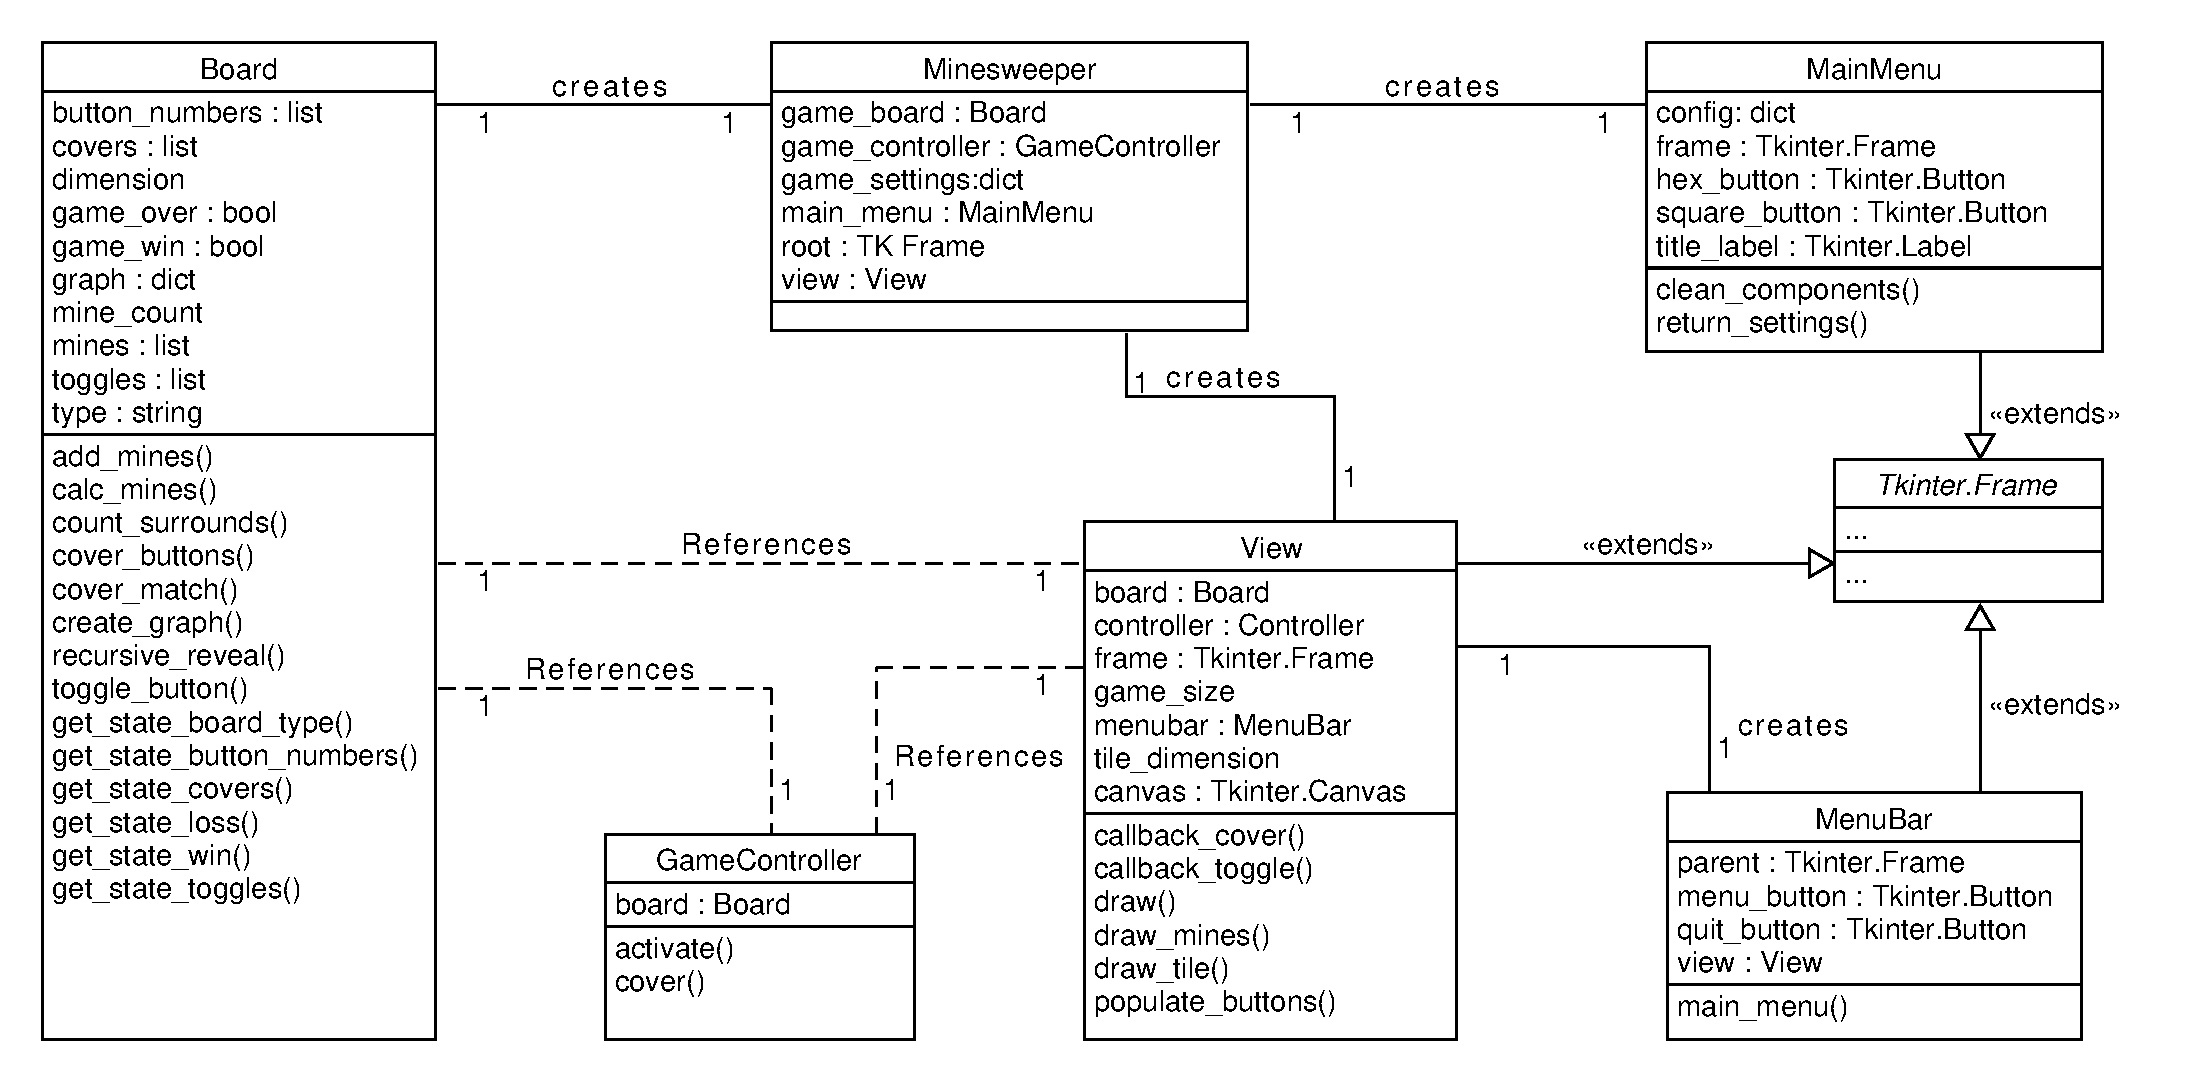
\includegraphics[scale=0.5]{ClassDiagram}
	\caption{UML class diagram for the Minesweeper software system}
	\label{ClassDiagram}
\end{figure}
\par Figure \ref{ClassDiagram} shows the overall structure of the software system including the methods and fields of each class, as well as the relationships between classes. It is evident in the class diagram that MVC principles are strictly adhered to as all code is separated into logically related sections. All code and information about the `model' or `game board' is stored within the board class. All user interface elements of the game are stored within the `view' class. As class diagrams are a structural model the related code has been included from various files in fragments below.

\begin{figure}[!h]
	\label{code:main}
	\begin{lstlisting}[language=python]
		self.game_board = Board(
			'square',
			self.game_settings['game_difficulty'],
			self.game_settings['game_size']
		);

		self.game_controller = GameController(self.game_board)

		self.view = View(self.game_board, self.game_controller, self.root, self.game_settings)
	\end{lstlisting}
	\caption{Extract from MineSweeper class}
\end{figure}

\par In the main class of the program `MineSweeper' an object of the game board is created. Then an object of the controller is created which has a reference to the game board. Finally an object of the view is instantiated with a reference to both the model `board' and the controller `Controller'. This is evident in figure 2.
\newline
\par It is observable in figure \ref{ClassDiagram} that the controller acts as a thin proxy or façade software pattern for the board class, abstracting the actual implementation from the view. In the code listing figure \ref{code:controller} it shows that the controller simply stores the reference to the model of the game as a member variable. The controller class also contains two small methods for performing different actions on the board model.
\begin{figure}[!h]
	\label{code:controller}
	\begin{lstlisting}[language=python]
		class GameController:
			def __init__(self, board):
				self.board = board
			
			def activate(self, i, j):
				print("[Controller] Passing", i, j,)
				self.board.toggle_button(i, j)
		
			def cover(self, i, j):
				print("[Controller] Covering", i, j)
				self.board.cover_button(i,j)
	\end{lstlisting}
	\caption{Extract from GameController class}
\end{figure}
\newline
\par The view object takes a reference to both the model and the controller as parameters and stores them as member variables. This allows the view to fetch the state of the board when drawing and to mutate the board through the controller when handling events. This is evident in the extract of the view class shown in figure 4.
\begin{figure}[!h]
	\label{view}
	\begin{lstlisting}[language=python]
		def __init__(self, game_board, game_controller, master, settings):
        	self.board = game_board
        	self.controller = game_controller
	\end{lstlisting}
	\caption{Extract from View class}
\end{figure}

\newpage
%
% ─── SEQUENCE DIAGRAM ───────────────────────────────────────────────────────────
%
\begin{figure}[!h]
	\centering
	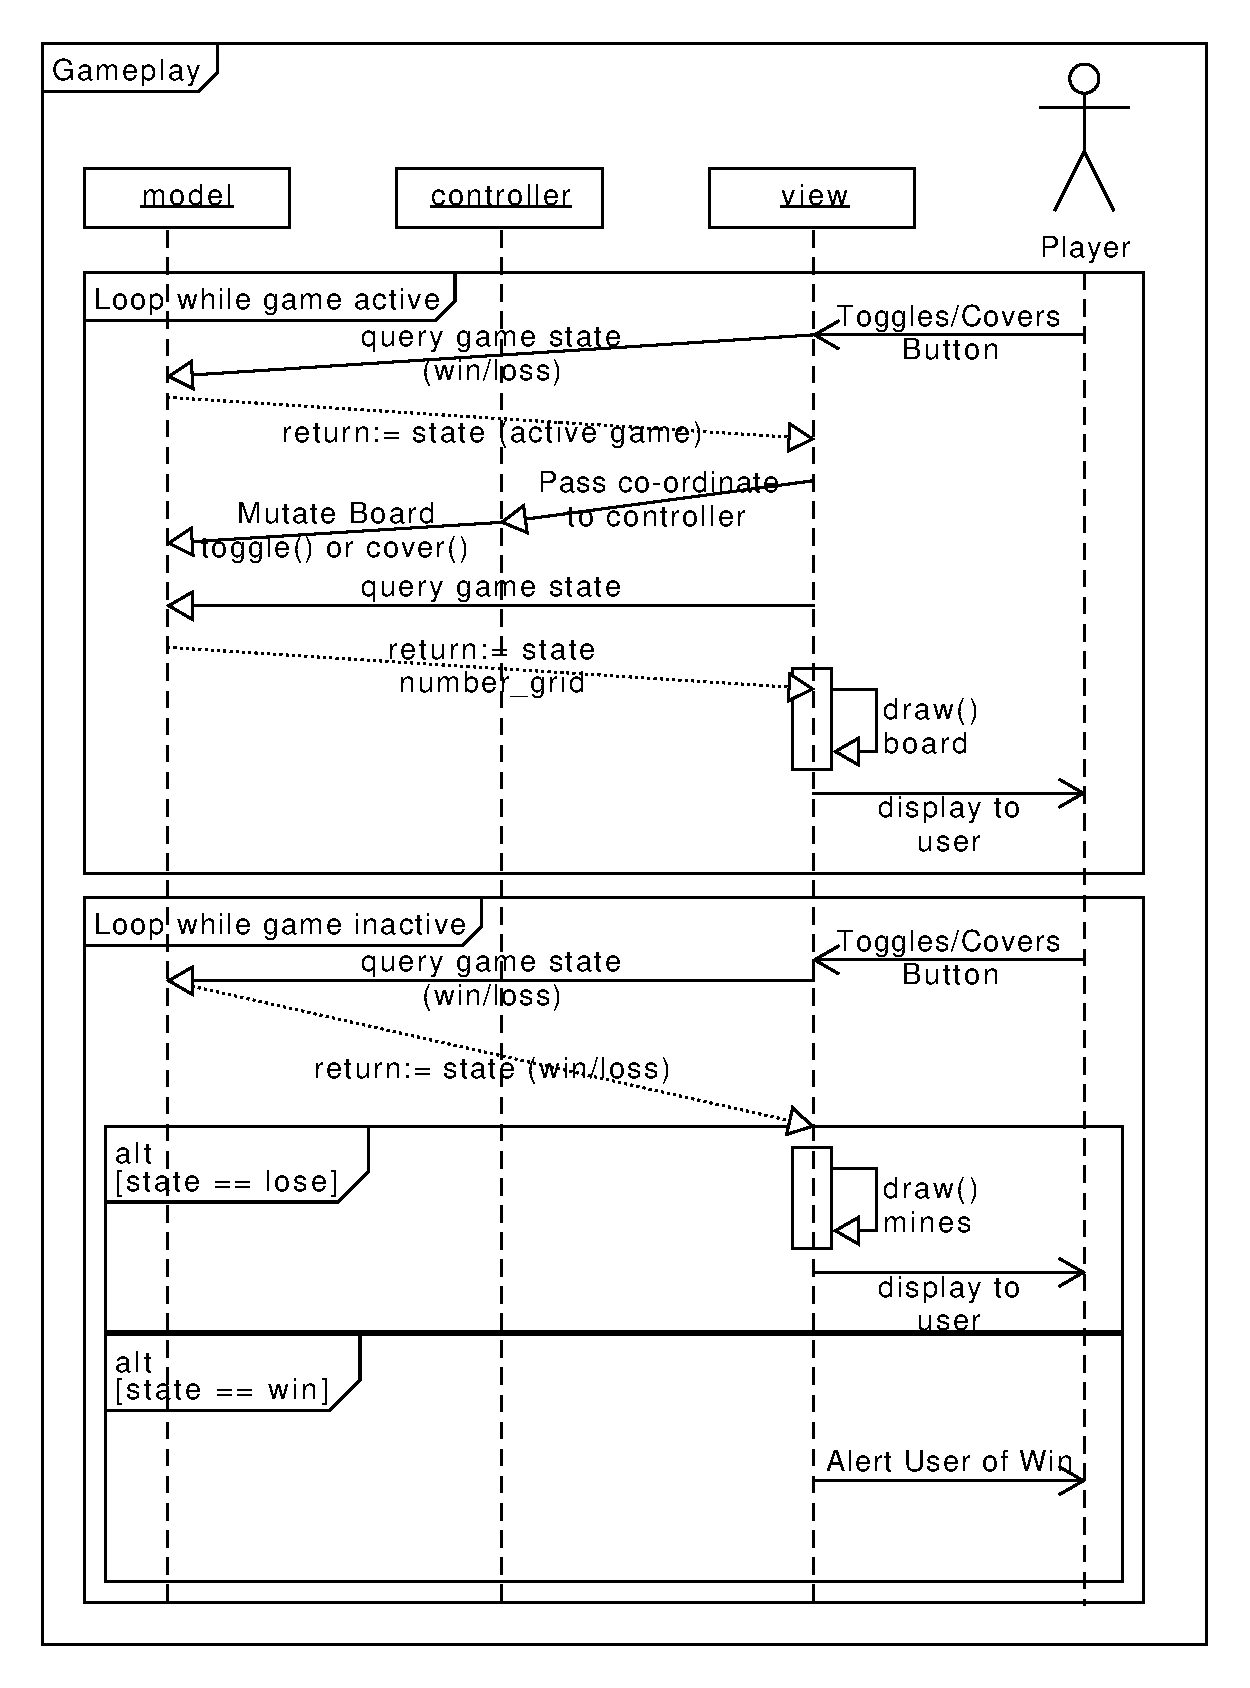
\includegraphics[scale=0.7]{SequenceDiagram}
	\caption{Sequence diagram for gameplay}
\end{figure}
Figure 5 is a sequence diagram which demonstrates how objects operate and interact with each other. Figure 5 demonstrates the interactions in the system during gameplay of minesweeper. It shows the user interacting with the user interface, the view calling the controller to mutate data and the view querying the state of the model after the model's state has changed. Figure 6 is an extract from the view class where the event handler passing information to the controller.
\begin{figure}[!h]
	\label{view}
	\begin{lstlisting}[language=python]
		def callback_toggle(self, event):
			#
			# --- DISABLE THE BOARD ON LOSS -----------------------------------
			if self.board.get_state_loss():
				return NONE
			if self.board.get_state_win():
				return NONE
			#
			# --- MUTATE THE BOARD THROUGH THE CONTROLLER ---------------------
			print("clicked at", event.x, event.y)
			button_i = event.x // 46
			button_j = event.y // 46
			print("clicked button: ", button_i, button_j)
			self.controller.activate(button_i, button_j)
			#
			# --- BEFORE REDRAW CHECK IF THE GAME IS OVER ---------------------
			if self.board.get_state_loss():
				self.draw_mines()
			else: 
				self.draw();

	\end{lstlisting}
	\caption{Extract from View class}
\end{figure}

\newpage
%
% ─── ACTIVITY DIAGRAM ───────────────────────────────────────────────────────────
%
\begin{figure}[!h]
	\centering
	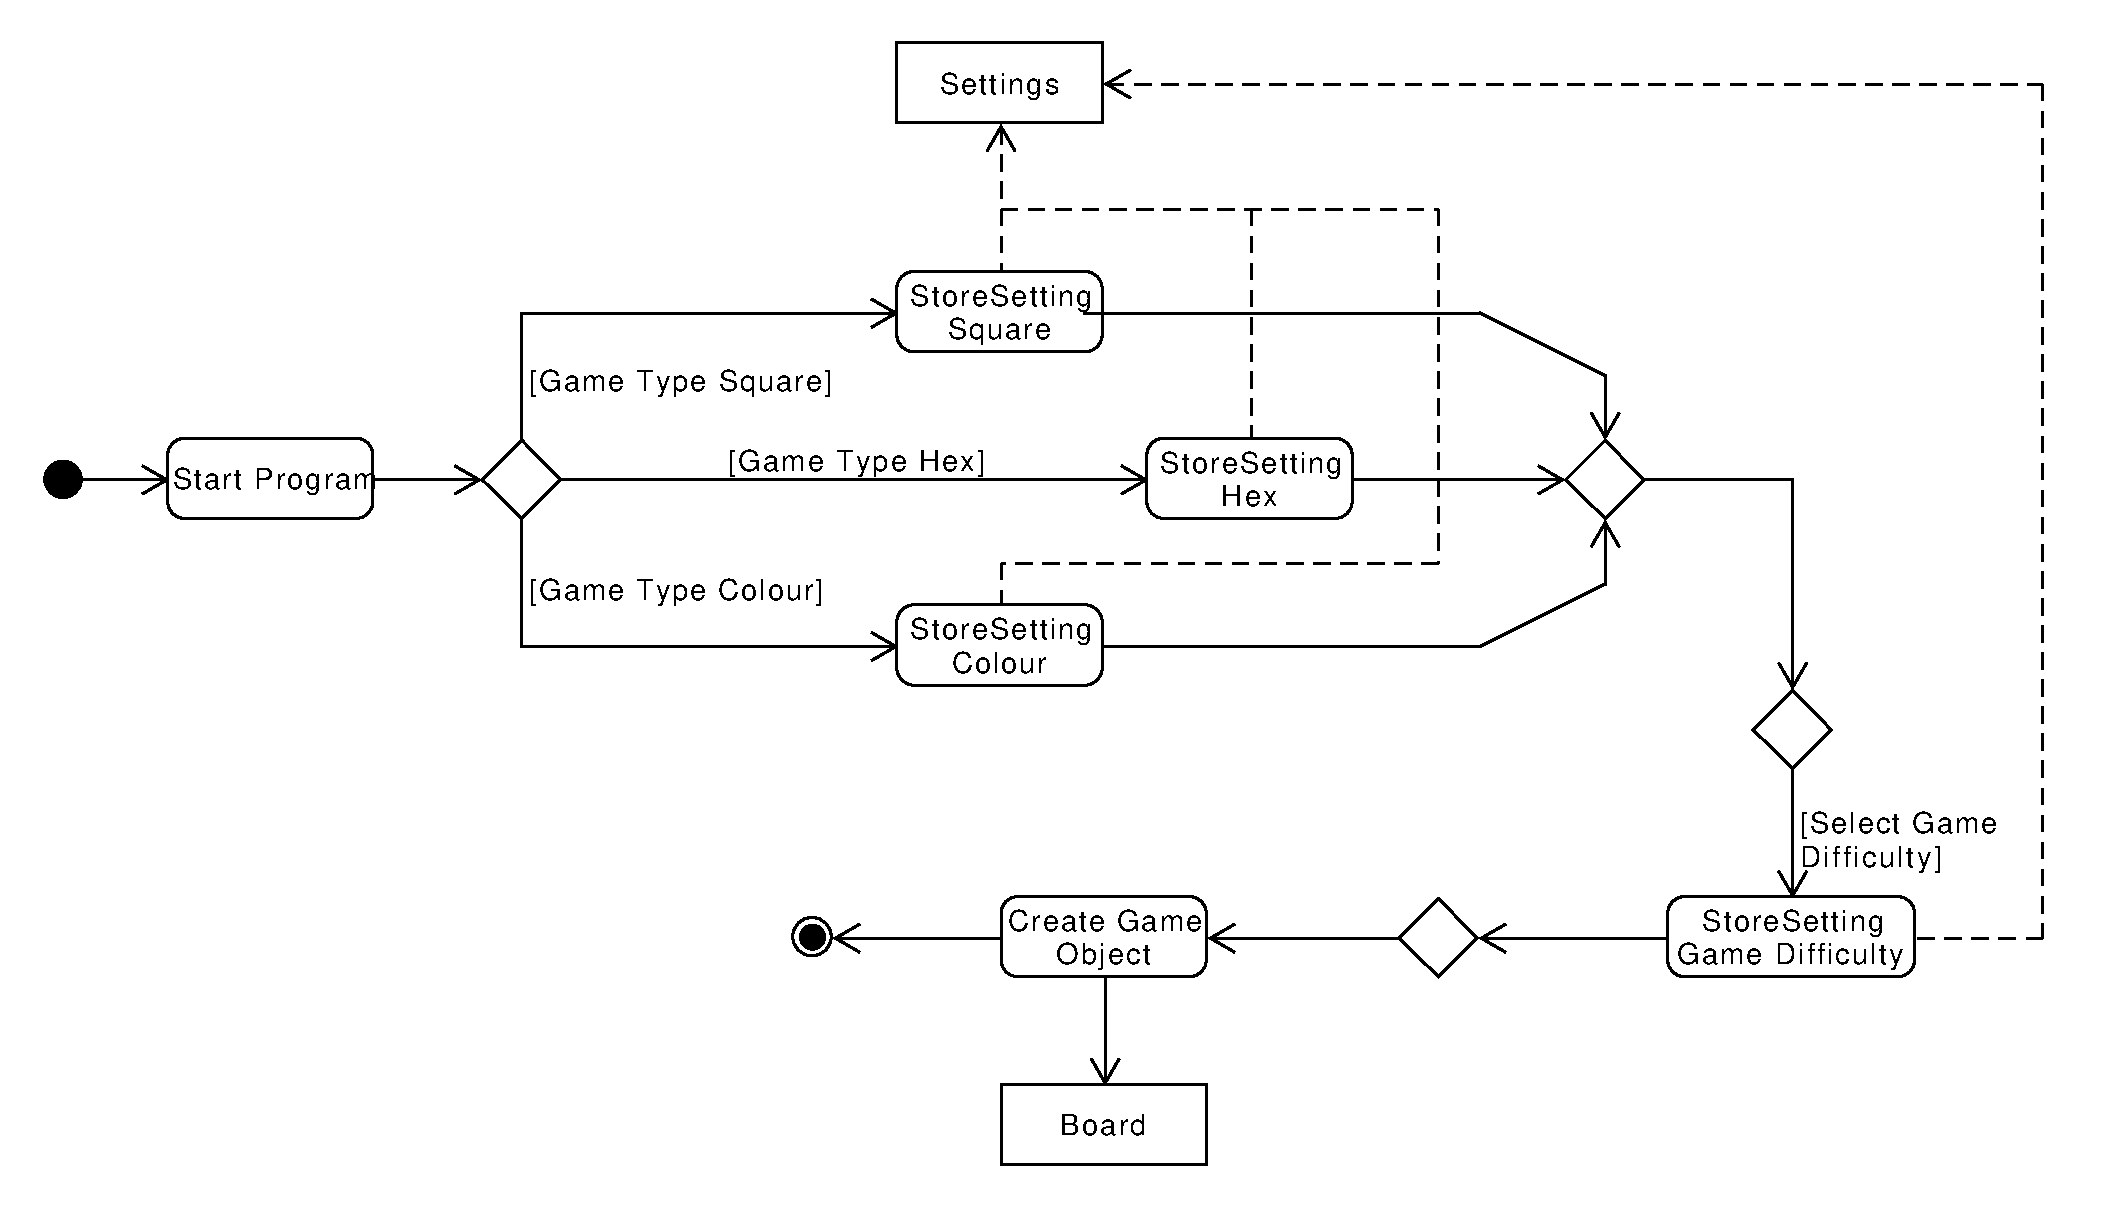
\includegraphics[scale=0.4]{ActivityDiagram}
	\caption{Activity diagram for MineSweeper}
\end{figure}
\par Figure 7 is an activity diagram and represents the program flow from one activity in the software system to another. Figure 7 visually represents the stages and decisions made when creating a new game. This activity diagram ends with the game being created and explains the storing of game settings and selection of game mode and difficulty. The following code extract in figure 8 shows the MainMenu object storing settings as key value pairs in a dictionary and then self closing. Figure 9 is code that shows how the settings are extracted to create a new board object.
\begin{figure}[!h]
	\label{view}
	\begin{lstlisting}[language=python]
		def return_settings(self, mode):
			self.clean_components()
			self.settings['mode'] = mode
			self.frame.destroy()
			self.frame.quit()
\end{lstlisting}
	\caption{Extract from MainMenu class}
\end{figure}
\begin{figure}[!h]
	\label{view}
	\begin{lstlisting}[language=python]
		self.game_board = Board(
			'square',
			self.game_settings['game_difficulty'],
			self.game_settings['game_size']
		);
\end{lstlisting}
	\caption{Extract from MineSweeper class}
\end{figure}

%
% ─── COLLABORATION DIAGRAM ──────────────────────────────────────────────────────
%
\begin{figure}[!h]
	\centering
	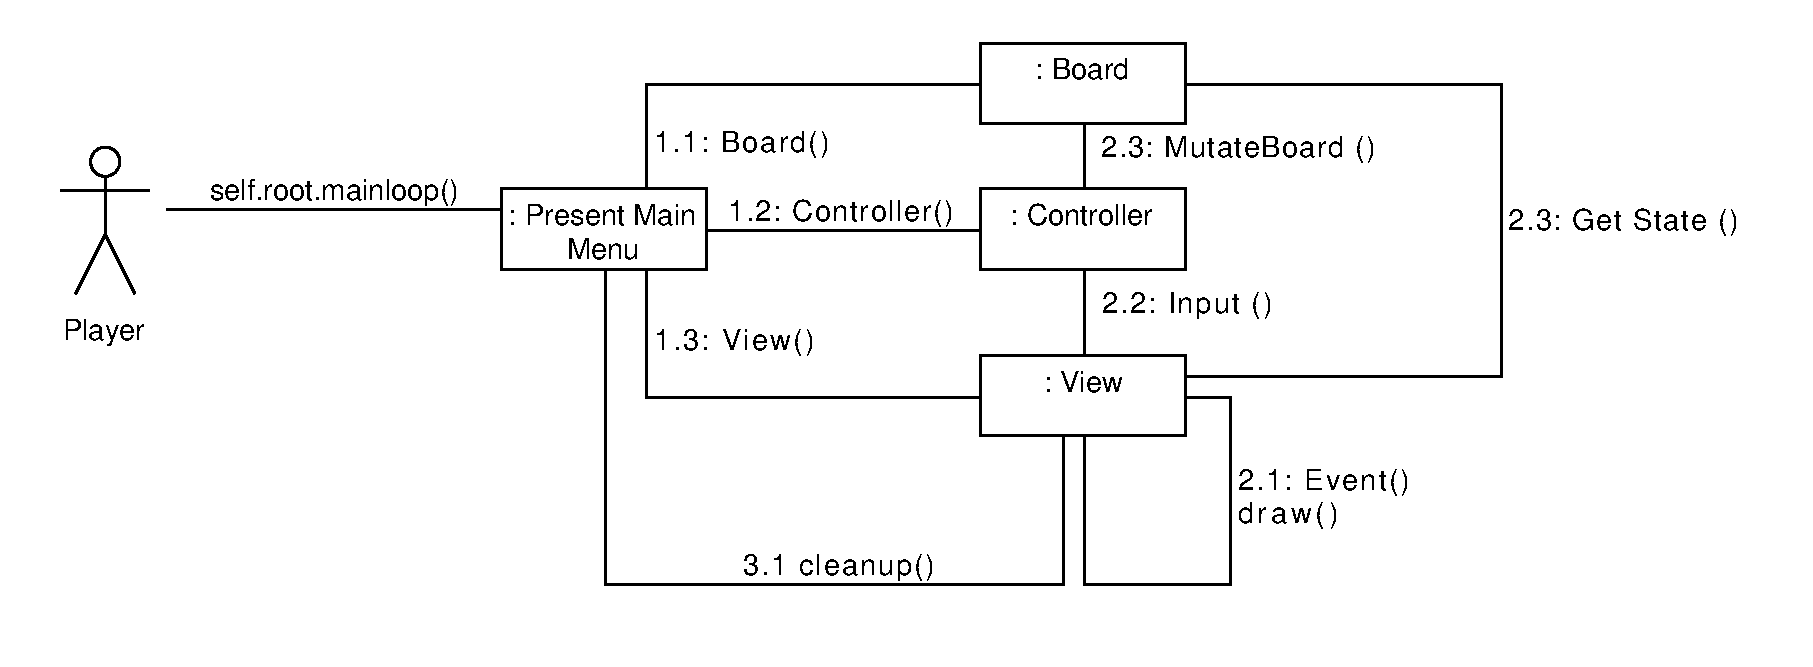
\includegraphics[scale=0.6]{CollaborationDiagram}
	\caption{Collaboration diagram for MineSweeper}
\end{figure}
\par Figure 10 is a collaboration diagram which illustrates relationships among objects. Figure 10 shows the object relationships when creating a new game. See figure 2 and figure 9.


\newpage
\subsection{Discussion of Sophistication Regarding Persistent Data Management, Access Control and User Interface}
\subsubsection{Persistent Data Management}
In the Minesweeper software system there is no persistent data stored in between games at this point in the game's development. Depending on your timeline there may be a need for a persistent data service in order to store user high scores. High scores are not a critical functional requirement and of the implementation of this data store is dependent on the workflow and time management of the developer.

\subsubsection{Access Control}
As there are no access restricted sections of the game and the software system currently only runs locally on a user's computer access control has not been a significant feature of the Minesweeper program. However, the security of the application is important as tampering could potentially put the user at risk. As the application does not run with root privileges and the user will be provided with a compiled binary, a security breach of the user's operating system or escalation of privileges is unlikely. As the software system is not exposed to the network remote security concerns do not need to be addressed within the scope of this product's development.

\subsubsection{User Interface}
The user interface for the software system of Minesweeper is quite sophisticated. It is built on top of the python tkinter library to create frames and components. The various sections of the user interface used in this application have been split into modules which subclass the tkinter frame object. This allows different UI components to be laid out in various configurations and increases maintainability as each component is limited in scope and functionality. This also enhances the re-usability of the code as models can be re-purposed in different situations. The user interface draws the tiles by rendering images onto a tkinter canvas object. This allows the game board to be very responsive and will make it easier to implement different views based on different configurations of the game by only changing a small subset of the code.

\newpage
\subsection{Software Testing \textbar{} Testing Plan \textbar{} Feasibility}
\par 


\begin{table}[!h]
\centering
\caption{Tests}
\label{my-label}
\begin{tabular}{lll}
Test Number & Test                                                          & Results     \\
1           & Selecting game mode returns correct value                     & \textcolor{codegreen}{As Expected} \\
2           & Specified mine density is represented on the board            & \textcolor{codegreen}{As Expected} \\
3           & Covers are not included in cascading reveal                   & \textcolor{codegreen}{As Expected} \\
4           & Cells that are already toggled cannot be covered              & \textcolor{codegreen}{As Expected} \\
5           & User cannot interact with the board after win                 & \textcolor{codegreen}{As Expected} \\
6           & user cannot interact with the board after game over           & \textcolor{codegreen}{As Expected} \\
7           & Recursive reveal also toggles a layer of 1's                  & \textcolor{codegreen}{As Expected} \\
8           & Mouse position is correctly converted to cell coordinates     & \textcolor{codegreen}{As Expected} \\
9           & Cell co-ordinates are passed in the right order to controller & \textcolor{codegreen}{As Expected} \\
10          & Game window resizes to fit the size of the game               & \textcolor{codegreen}{As Expected} \\
11          & Game window cannot be resized manually                        & \textcolor{codegreen}{As Expected} \\
12          & Quit button gracefully exits                                  & \textcolor{codegreen}{As Expected} \\
13          & Main menu button cleans the view and returns to main menu     & \textcolor{codegreen}{As Expected} \\
14          & Winning requires correct covers                               & \textcolor{codegreen}{As Expected} \\
15          & Game loses when clicking a mine                               & \textcolor{codegreen}{As Expected} \\
16          & Game is responsive up to 25n dimension                        & \textcolor{codegreen}{As Expected}
\end{tabular}
\end{table}

\subsection{Version Control}
\par The version control used in developing this software system was Git. And the source repository was hosted on the website GitHub.com. This allowed for the generation of graphs as well as logs of commits and other metrics. By using version control the project has been able to accurately track the source code as well as providing valuable versioning services used when trying to determine when a bug was introduced into the source. As the developers work across multiple devices source control has been a valuable tool in keeping multiple local copies of the repository synchronized and up-to-date across multiple computers.

		% \subsubsection{Version Control History / Log}
\begin{table}[!h]
\centering

\begin{tabular}{llp{9cm}}
Time				  & Author   & Comment \\ \hline
Sun Sep 3 14:56 2017  & ZaymonFC & Added all diagrams \\
Sun Sep 3 00:19 2017  & ZaymonFC & Added Histogram and Activity Diagram \\
Sat Sep 2 23:26 2017  & ZaymonFC & Added sequence diagram \\
Sat Sep 2 22:40 2017  & ZaymonFC & Added class diagram \\
Sat Sep 2 21:26 2017  & ZaymonFC & Added 5 sections to report \\
Sat Sep 2 18:29 2017  & ZaymonFC & Added encoding for epydoc2 \\
Sat Sep 2 18:27 2017  & ZaymonFC & Added encoding for epydoc \\
Sat Sep 2 17:00 2017  & ZaymonFC & Added Report Dir \\
Fri Sep 1 23:17 2017  & ZaymonFC & Added Covers \\
Fri Sep 1 22:59 2017  & ZaymonFC & Implementing covers \\
Fri Sep 1 22:42 2017  & ZaymonFC & Implemented MVC and used canvas to draw board \\
Fri Sep 1 18:49 2017  & ZaymonFC & Merge branch `master' of https://github.com/ZaymonFC/PSD\_MineSweeper \\
Fri Sep 1 18:49 2017  & ZaymonFC & PreMerge \\
Fri Sep 1 18:02 2017  & ZaymonFC & Added click position event hadler for game canvas \\
Fri Sep 1 16:37 2017  & ZaymonFC & Added function to render grid of buttons to canvas \\
Fri Sep 1 15:43 2017  & ZaymonFC & Added view \\
Wed Aug 30 22:36 2017 & ZaymonFC & Added title lable and finished main menu functionality \\
Wed Aug 30 21:25 2017 & ZaymonFC & Added button assets for main menu and worked on GUI components \\
Wed Aug 30 20:27 2017 & ZaymonFC & Added skeleton for MVC \\
Wed Aug 30 19:09 2017 & ZaymonFC & Started Game Restructure \\
Mon Jul 31 20:07 2017 & ZaymonFC & Modified recursive reveal to show extra layer of tiles \\
Fri Jul 28 23:45 2017 & ZaymonFC & Fixed button tile images to display actual tile png' 
\end{tabular}
\end{table}

\begin{table}[!h]
\centering	
\begin{tabular}{ll p{9cm}}
Fri Jul 28 20:02 2017 & ZaymonFC & Added Class Diagram Data \\
Fri Jul 28 19:59 2017 & ZaymonFC & Added Class Diagram \\
Fri Jul 28 19:31 2017 & ZaymonFC & MileStone 01 Achieved \\
Fri Jul 28 17:08 2017 & ZaymonFC & Added recursive reveal and reveal mine end conditions \\
Fri Jul 28 16:34 2017 & ZaymonFC & Added images for python implementation and added event callbacks to the buttons \\
Thu Jul 27 23:45 2017 & ZaymonFC & Added grid of buttons with colouring to test generating functions \\
Thu Jul 27 23:25 2017 & ZaymonFC & Added methods to the python variant to create the graph, add the mines and generate the button numbers \\
Thu Jul 27 22:39 2017 & ZaymonFC & Modified Tiles,  Created a python attempt at back end representation \\
Thu Jul 27 20:57 2017 & ZaymonFC & Merge branch `master' of https://github.com/ZaymonFC/PSD\_MineSweeper \\
Thu Jul 27 20:57 2017 & ZaymonFC & MineSweeperJS Fixed \\
Wed Jul 26 12:32 2017 & ZaymonFC & Worked on creating the graph for neighbors \\
Tue Jul 25 15:28 2017 & ZaymonFC & Added style and untracked output files from main repo \\
Tue Jul 25 15:14 2017 & ZaymonFC & Added square tile spritesheet and frameboarder \\
Tue Jul 25 14:46 2017 & ZaymonFC & Fixed index title,  added a class for game tile which extends the phaser button object \\
Tue Jul 25 00:11 2017 & ZaymonFC & Added assets for buttons,  loaded them into the mainmenu game state and then created event handlers to switch state to the GameState class\\
Mon Jul 24 23:38 2017 & ZaymonFC & Added Mainmenu state,   fixed state handling,  implemented a global constant file for game configurations \\
Mon Jul 24 23:00 2017 & ZaymonFC & Setup webpack and refactored starting code. Added MineSweeper class to act as a state manager \\
Mon Jul 24 20:10 2017 & ZaymonFC & Configured node modules and installed webpack \\
Mon Jul 24 20:00 2017 & ZaymonFC & Created class to represent tile and created basic constructor \\
Sun Jul 23 22:36 2017 & ZaymonFC & Understood working with phaserjs sprites and implemented a `game' GameState \\
Sun Jul 23 14:02 2017 & ZaymonFC & Initial Commit
\end{tabular}
\end{table}

\newpage
\clearpage
\subsubsection{Histogram of Effort}
\begin{figure}[!h]
	\centering
	\includegraphics[scale=1]{Histogram}
	\caption{Collaboration diagram for MineSweeper}
\end{figure}

\par It is evident from figure 11 that the effort distribution is skewed towards the submission of each milestone. This is due to the developers prioritizing time based on assessment due dates.

	
	% 	\par\vspace{1cm}\small Note: Repository is private to prevent plagiarism. \textbar{} This log was created by using the command \begin{lstlisting} 
	% 	git log --pretty=format:`%h;%an;%s' > ./log.csv\end{lstlisting}
	
	
	
\end{document}

